\documentclass[12pt, a4paper]{article} %,twoside

\usepackage[literat, microtype, nocolor]{derradeiro}




\begin{document}

\noindent\rule{\textwidth}{0.4pt}
Недавние археологические открытия выявили, что парламент функционировал несмотря на приверженности законодателей к странствованиям. Законодатели поддерживали копии записей парламента согласованными, несмотря на их частые уходы по важным делам и забывчивость посыльных. Протокол парламента паксонов представляет новый способ реализации автоматного подхода в дизайне распределённых систем.\\
\noindent\rule{\textwidth}{0.4pt}

Представленное было обнаружено недавно за систематизацией материалов в офисе редакции TOCS. Несмотря на древность, главный редактор считал, что материал не стоит публикации. Так как автор был занят работой на греческих островах и не был достижим, меня попросили подготовить этот материал.

Автором работы был археолог, который лишь немного интересовался компьютерными науками. К сожалению; ведь даже при условии, что цивилизация Паксон была мало изучена и непонятна, как описывает автор, их законодательная система --- это исключительный пример того, как можно реализовать распределённую систему, работающую в асинхронной среде. Действительно, набор усовершенствований добавленных жителями Паксон в свой протокол оказался не известным в технической литературе.

Автор даёт краткое описание связи Парламента цивилизации Паксон и распределённых вычислений в секции \ref{sec:csconnection}. Информатики возможно захотят прочитать эту секцию в первую очередь. И даже раньше они могут обратиться к объяснению алгоритма для информатиков автора Lampson[1996]. Более формально алгоритм описан De Prisco [1997]. Я также добавил дополнительные комментарии о связи древнего протокола и более современных разработок в конце четвертой секции.

\begin{flushright}
Keith Marzullo

Калифорнийский университет, Сан Диего
\end{flushright}

\newpage
\section{Проблема}
\subsection{Остров Паксос}

В начале тысячелетия, Эгейский остров Паксос был процветающим торговым центром. Богатство привело к политическому совершенству, и паксоны заменили древнюю теократию парламентской формой правления. Однако торговля всё же стояла на первом месте по отношению к политической ответственности и ни один паксон не горел желанием посвятить свою жизнь парламенту. Парламент должен был функционировать даже при условии, что законодатели постоянно то уходили, то приходили в законодательную палату.

Проблема управления парламентом с частичной занятостью оказывается удивительно схожей с актуальной проблемой создания отказоустойчивых распределённых систем, где законодатели соответствуют процессам, а покидание парламента --- ошибке при обработке. Решение паксонов может заинтересовать информатиков. Я представляю небольшой исторический рассказ о протоколе парламента Паксон, продолжаемый ещё более коротким описанием его отношения к распределённым системам.

Цивилизация Паксон была уничтожена иностранным вторжением, и только недавно археологи начали докапываться до их истории. Наши знания об их парламенте в силу этих обстоятельств достаточно фрагментарны. Несмотря на то, что базовый протокол известен, мы очень плохо осведомлены о многих деталях. Тогда как именно эти детали представляют наибольший интерес. Я возьму на себя ответственность за предположения о том, что же в действительности совершили паксоны.

\subsection{Требования}

Главной задачей парламента являлось определение закона страны, образуемого последовательностью принятых декретов. В современном парламенте наняли бы секретаря для их записи, но на острове Паксос не было ни одного желающего на протяжении всей сессии находиться в Палате и выполнять эту роль. Вместо этого, каждый законодатель хранил \textit{книгу учёта} в которой делал нумерованные записи принятых декретов. Например, в книге законодателя $\Lambda\iota\nu\chi\partial$ находилась запись:
\centerblock{
    155: Налог на оливки составляет 3 драхмы за тонну
}
если они считала, что 155 декрет парламента был принят и устанавливал размер налога на тонну оливок в 3 драхмы. В книгах писали несмываемыми чернилами и записи в них нельзя было изменить.

Первое требование протокола парламента заключалось в корректности записей в учётных книгах, означающей, что не в каких двух книгах не могло быть противоречивой информации. Если законодатель $\Phi\iota\partial\epsilon\rho$ хранил в своей книге запись 
\centerblock{
    132: Лампы должны использовать только оливковое масло
}
то никто другой не мог хранить другую запись для декрета с номером 132. Однако другой законодатель мог под этим номером записи не иметь, если он не знал был ли такой декрет принят.

Согласованность книг учёта была недостаточной, так как они могли быть попросту все пустыми. Необходимо было такое требование, которое бы гарантировало, что декреты в конце концов всё-таки были бы приняты и записаны в книги. В современном парламенте, препятствием к принятию декрета является несогласие среди законодателей. Но такого не было среди паксонов, среди которых  атмосфера взаимного доверия преобладала. Законодатели паксонов имели желание принять каждый декрет, выносимый на рассмотрение. Но странствующий уклад жизни был проблемой. Согласованность была бы потеряна, если бы одна группа законодателей приняла декрет 
\centerblock{ 
    37: Рисовать на стенах храма запрещено
}
а потом ушла на банкет, в то время как другая группа посетила зал заседания и, не зная ничего о том, что произошло, приняла противоречащий закон 
\centerblock{
    37: Свобода художественного самовыражения гарантирована
}

Прогресс не мог быть гарантирован, пока достаточное число законодателей не оставалось в палате достаточное количество времени. Потому как законодатели паксонов не хотели сокращать свои дела не связанные с парламентом, быть уверенным, что когда-нибудь будет принят какой-либо декрет было невозможно. Однако, законодатели желали гарантировать, что находясь в палате, они и их помощники будут действовать без промедлений по всем вопросам парламента. Эта гарантия позволяла вывести протокол парламента, удовлетворяющий следующему условию прогресса:

    Если большинство законодателей\footnote{При переводе условия прогресса, я поставил в соответствие слову паксонов $\mu\alpha\delta\zeta\partial\omega\rho\iota\tau\check{\iota}\sigma\epsilon\tau$ перевод \textit{большинство законодателей} (majority of legislators). Альтернативные переводы этого слова предложены и обсуждаются в секции \ref{sec:preliminaryprot}} находились в палате и никто не покидал или входил в палату в течении достаточно долгого периода времени, тогда любой декрет, вынесенный на рассмотрение будет принят и окажется записан во все книги учёта всех законодателей в палате.

\subsection{Допущения}

Требования протокола парламента могли быть удовлетворены только при обеспечении законодателей всеми необходимыми ресурсами. Каждый законодатель получал здоровую книгу для записи декретов, ручку и запас несмываемых чернил. Законодатели могли забывать что они делали после ухода из палаты, поэтому они делали записи о важных задачах в конце книги. Строку в списке декретов нельзя было изменить, но записи в конце можно было спокойно вычеркнуть. Для достижения условия прогресса необходимо было, чтобы законодатели могли измерять количество прошедшего времени, и для этого им выдавались простые песочные часы.

Законодатели таскали свои книги всё время и могли всегда прочитать список декретов и любую незачёркнутую запись. Листы книги были изготовлены из тончайшего пергамента, поэтому использовались для самых важных записей. Законодатель мог записать менее важные вещи на листке бумаги, который он мог (или не мог) потерять, когда уходил из парламента.

С той акустикой зала, которая была в палате ораторствовать было совершенно невозможно. Заседающие могли общаться только через посыльных и были снабжены достаточным количеством денег для найма такого их количества, которое им было нужно. Посыльный должен был учесть, что не может исказить сообщение, но ему позволялось забыть, что он только что доставил сообщение и передать его заново. Как и законодатели, посыльные посвящали работе в парламенте только часть времени. Посыльный мог покинуть палату по важному делу, например шестимесячное путешествие, прежде чем доставить сообщение. Он мог также больше никогда не возвращаться, что таким образом делало сообщение потерянным.

Хотя законодатели и посыльные могли приходить и уходить в любое время, в пределах палаты они посвящали всё работе связанной с парламентом. Многие специалисты не верят этому всерьёз, считая эту информацию пропагандой, чтобы изобразить Паксос как землю с более высокими моральными ценностями, чем соседи на востоке. Нечестность, хоть и редко, конечно же была. Однако, в силу того, что ни в одном официальном документе об этом не упоминается, мы имеем слабое представление о том, как они справлялись с нечестным поведением законодателей и посыльных. В секции \ref{sec:evilorholy} будет описаны факты, к которым мы пришли.

\section{Синод одного декрета}

Парламент Паксон эволюционировал из раннего церемониального Синода жрецов, который собирался каждые 19 лет для выбора единого, воплощенного в записи декрета. На протяжении многих веков Синод выбирал декрет процедурой голосования, требующей присутствия всех жрецов. Но по мере процветания торговли, жрецы стали то уходить, то приходить в Палату во время заседания. В конце концов, старый протокол дал сбой и заседание окончилось без принятого декрета. Чтобы предотвратить повторения теологической катастрофы, лидеры цивилизации паксон обратились к математикам, чтобы они сформулировали протокол выбора декрета Синода. Требования и допущения протокола были по существу такими же, какие использовались в будущем Парламенте, за исключением того, что книга содержала один декрет вместо нескольких. Окончательный протокол Синода описан далее, а протокол парламента в секции \ref{sec:parlamentprot}.

Математики выводили протокол Синода в несколько шагов. Во-первых, они доказали, что протокол, удовлетворяющий набору ограничений будет гарантировать согласованность  и прогресс. \textit{Предварительный протокол} (\textit{preliminary protocol}) был выведен следом из этого набора ограничений. Ограниченная  версия предварительного протокола, \textit{базовый протокол} (\textit{basic protocol}), гарантировала согласованность, но не прогресс. Завершённый протокол Синода, удовлетворяющий требованиям согласованности и прогресса был получен из базового вводом дополнительных ограничений\footnote{Подробная история создания протокола Синода не известна. Как современные информатики, математики паксонов описывали элегантные, логические выводы, которые не имели ничего общего с тем, как выводят алгоритмы. Однако, известно, что результаты математиков (Теорема 1 и 2 из секции \ref{sec:mathsupport}) действительно предшествовали протоколу. Они были выведены, когда математики, в ответ на запрос создания протокола, попытались доказать, что такого протокола не существует.
}.

\subsection{Результаты математиков}\label{sec:mathsupport}

Декрет Синода выбирался серией пронумерованных \textit{бюллетеней} (\textit{ballot}), где бюллетень был результатом референдума одного декрета. В каждом бюллетене, жрец мог только либо проголосовать за декрет или проигнорировать его\footnote{Как и некоторые современные нации, Паксос не полностью понимали природу Афинской демократии.}. Ассоциированное с каждым бюллетенем множество называлось \textit{кворумом} (\textit{quorum}). Бюллетень считался успешным тогда и только тогда, когда каждый жрец в кворуме проголосовал за декрет.  Формально, бюллетень $B$ состоял из 4-х компонентов. (Пока не определено обратное, \textit{множество} обозначает \textit{конечное множество}\footnote{Несмотря на то, что математики паксон были очень развитым для того времени, они очевидно не имели знаний о теории множеств. Я взял на себя ответственность в переводе более примитивной нотации в язык современной теории множеств}.)
\begin{table}[h]
\begin{tabular}{ l p{10.5cm}}
    $B_{dec}$ & Декрет (тот, за который проголосовали)\\
    $B_{qrm}$ & Непустое множество жрецов (кворум бюллетеня)\\
    $B_{vot}$ & Набор жрецов (тех, которые голосуют за декрет)\footnote{Только жрецы кворума действительно голосовали, но математики паксон выяснили, что будет проще убедить людей, что протокол верен, если в их доказательстве они позволят голосовать любому жрецу за любой бюллетень.}\\
    $B_{bal}$ & Номер бюллетеня
\end{tabular}
\end{table}

Бюллетень $B$ назывался \textit{успешным} тогда и только тогда, когда $B_{qrm} \subseteq B_{vot}$ так, что успешный бюллетень соответствует тому, за который проголосовали все члены кворума.

Номера бюллетеней выбирались из бесконечного упорядоченного множества чисел. Если $B_{bal}' > B_{bal}$, тогда бюллетень $B'$ назвался более поздним, чем $B$. Однако, это никак не отражало тот порядок, в котором бюллетени обрабатывались; более поздний бюллетень мог быть обработан перед ранним.

Математики паксон определили 3 ограничения над множеством $\mathcal{B}$ бюллетеней и далее показали, что обеспечивается согласованность, а прогресс может иметь место, если обрабатываемое множество бюллетеней соответствовало этим ограничениям. Первые два ограничения были простыми; они могут быть сформулированы неформально следующим образом.
\begin{table}[h]
\begin{tabular}{l p{10.5cm}}
    $B1(\mathcal{B})$ & Каждый бюллетень в $\mathcal{B}$ обладает уникальным номером.\\
    $B2(\mathcal{B})$ & Кворумы любых двух бюллетеней в $\mathcal{B}$ включают хотя бы одного общего жреца.
\end{tabular}
\end{table}

Третье ограничение было более сложным. Один манускрипт паксонов содержал следующее, достаточно запутанное утверждение.
\begin{table}[h]
\begin{tabular}{l p{10.5cm}}
    $B3(\mathcal{B})$ & Для каждого бюллетеня $B$ в $\mathcal{B}$, если любой жрец в кворуме голосовал за \textit{предыдущий} бюллетень в $\mathcal{B}$, тогда декрет $B$ эквивалентен декрету последнего бюллетеня из ранних бюллетеней. 
\end{tabular}
\end{table}

Интерпретация этого загадочного текста облегчалась манускриптом, изображённым на Рисунке 1, который иллюстрирует условие $B3(\mathcal{B})$ с множеством $\mathcal{B}$ из пяти бюллетеней для Синода, состоящего из пяти жрецов $A$, $B$, $\Gamma$, $\Delta$ и $E$. Это множество $\mathcal{B}$ состоящее из пяти бюллетеней, где для каждого бюллетеня, множества проголосовавших --- подмножество жрецов кворума, чьи имена заключены в рамки. Например, номер бюллетеня 14 содержал декрет $\alpha$, кворум, состоящий из трёх жрецов и множества из двух голосующих. Условие $B3(\mathcal{B})$ имело вид <<для каждого $B$ в $\mathcal{B}$: $\ldots$>>, где <<$\ldots$>> --- это условие бюллетеня $B$. Условия пяти бюллетеней $B$ Рисунка \ref{fig:paxonmanu} следующие.

\begin{figure}[h]
 \centering
    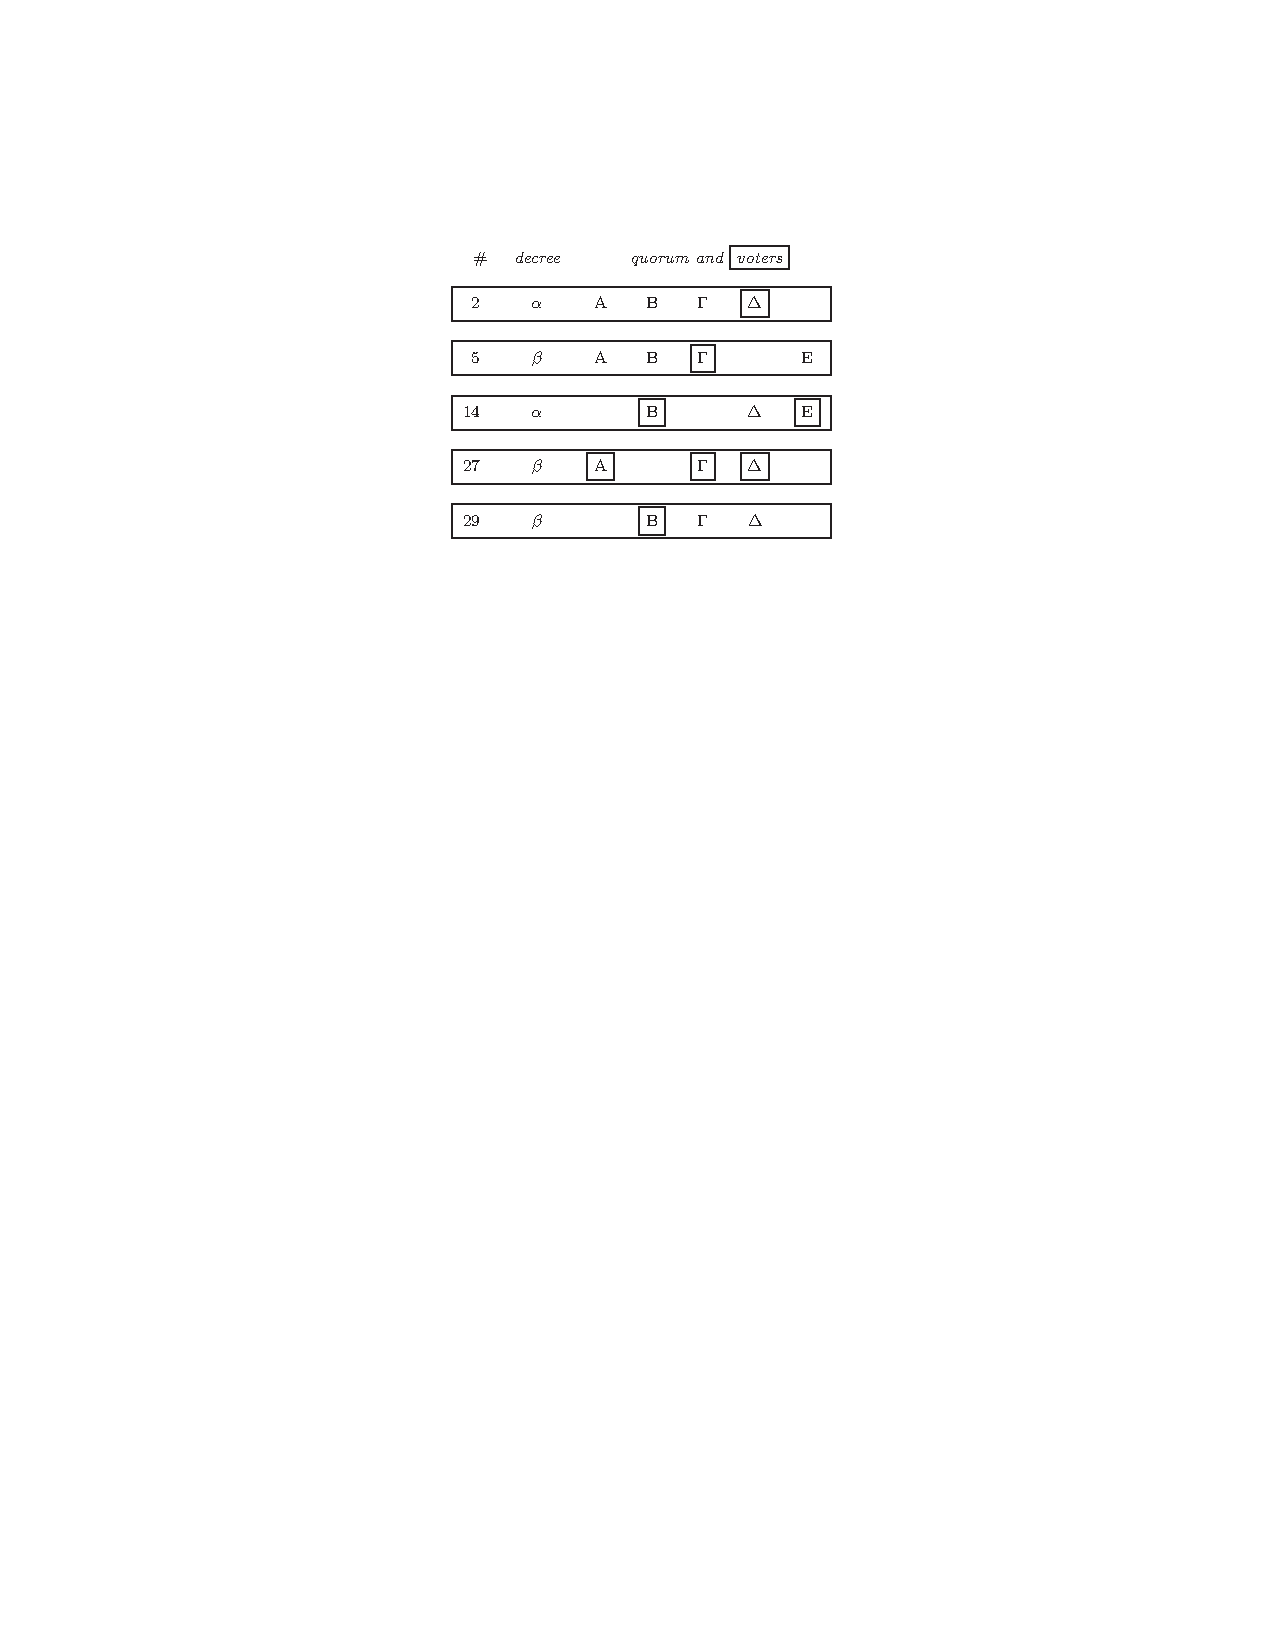
\includegraphics[width=0,8\textwidth]{images/Paxon-manuscript.pdf}
    \caption{Манускрипт паксонов.}
    \label{fig:paxonmanu}
\end{figure}

\begin{itemize}
    \item[2.] Бюллетень с номером 2 --- самый ранний бюллетень, поэтому его ограничение заведомо верное.
    \item[5.] Ни один из членов кворума бюллетеня под номером 5 не голосовал за ранний, так что ограничение также верно.
    \item[14.] Единственный член бюллетеня 14, который голосовал за предыдущие это $\Delta$, проголосовавший за номер 2, так что условие требует, чтобы декрет 14 бюллетеня был также декретом 2-ого.
    \item[27.] (Успешный бюллетень.) Члены кворума 27-ого бюллетеня: $A$, $\Gamma$ и $\Delta$. Жрец $A$ не голосовал за ранние бюллетени, единственный ранний бюллетень за который голосовал $\Gamma$ это 5-ый, а $\Delta$ оставил голос за 2. Последний из этих двух бюллетеней --- пятый, таким образом согласно ограничению декрет 27-ого бюллетеня должен совпадать с декретом под номером 5.
    \item[29.] Члены кворума бюллетеня 29: $B$, $\Gamma$ и $\Delta$. $B$ уже один раз проголосовал за 14, жрец $\Gamma$ за 5 и 27, а $\Delta$ голосовал за 2-й и 27-й. Самый поздний из четырёх бюллетений --- 27, поэтому условие требует, чтобы 29 декрет совпадал с 27.
\end{itemize}


Чтобы утверждать $B1(\mathcal{B}) - B3(\mathcal{B})$ формально требуется дополнительная нотация (определения). \textit{Голос} $v$ был определён как элемент, состоящий из трёх компонетов: жреца $v_{pst}$, бюллетеня $v_{bal}$ и декрета $v_{dec}$. Он представляет голос осуществлённый жрецом $v_{pst}$ за декрет $v_{dec}$ в бюллетене $v_{bal}$. паксоны также ввели $null$ голоса, такие, что $v_{bal}=-\infty$ и $v_{dec}=\mathrm{BLANK}$, где $-\infty < b < \infty$ для любого номера бюллетеня $b$ и $\mathrm{BLANK}$ не являющийся декретом. Для любого жреца $p$, они ввели $null_p$ как уникальный голос $v$, где $v_{pst}=p$.

Математики Пакcон определили полное упорядочение над множеством всех голосов, но часть манускрипта, содержащая эту информацию была утеряна. Сохранившийся фрагмент подсказывает, что для любого голоса $v$ и $v'$, при условии, что $v_{bal} < v_{bal}'$ выполняется $v < v'$. Нет информации о том, в каком порядке идут $v$ и $v'$, если $v_{bal} = v_{bal}'$.

Для любого множества $\mathcal{B}$, множество $Votes(\mathcal{B})$ голосов в $\mathcal{B}$ было определено состоящим из голосов $v$, таких, что $v_{pst} \in B_{vot}$, $v_{bal} = B_{bal}$ и $v_{dec} = B_{dec}$ для некоторых $B \in \mathcal{B}$. Если $p$ --- жрец, а $b$ номер бюллетеня или $\pm \infty$, тогда $MaxVote(b, p, \mathcal{B})$ было определено как максимальный голос из $Votes(\mathcal{B})$ совершённый $p$ c $v_{bal} < b$, или было равным $null_p$, если такого голоса не существовало. Так как $null_p$ меньше чем любой реально осуществлённый голос $p$, то $MaxVote(b,p, \mathcal{B})$ --- это максимальный голос из множества:
\[  
    \{v \in Votes(\mathcal{B}) : (v_{pst} = p) \land (v_{bal} < b)\} \cup \{null_p\}
\]
Для любого не пустого множества жрецов $Q$, $MaxVote(b, Q, \mathcal{B})$ был определён равным как максимум всех голосов $MaxVote(b, p, \mathcal{B})$ с $p$ в $Q$.

Ограничения  $B1(\mathcal{B}) - B3(\mathcal{B})$ утверждаются формально следующим образом\footnote{Я использую обозначение математиков паксонов $\overset{\Delta}{=}$, означающее \textit{тождественно равно}.}:
\begin{align*}
    &B1(\mathcal{B}) \overset{\Delta}{=} \forall B, B' \in \mathcal{B} : (B \neq B') \Rightarrow (B_{bal} \neq B_{bal}') \\
    &B2(\mathcal{B}) \overset{\Delta}{=} \forall B, B' \in \mathcal{B} : B_{qrm} \cap B_{qrm}' \neq \emptyset \\
    &B3(\mathcal{B}) \overset{\Delta}{=} \forall B \in \mathcal{B} : (MaxVote(B_{bal}, B_{qrm}, \mathcal{B})_{bal} \neq - \infty) \Rightarrow \\
    &(B_{dec} = MaxVote(B_{bal}, B_{qrm}, \mathcal{B})_{dec}) \\
\end{align*}
Несмотря на то, что определение $MaxVote$ зависит от порядка голосов, $B1(\mathcal{B})$ влечёт за собой то, что $MaxVote(b, Q, \mathcal{B})_{dec}$ не зависит от порядка голосов с эквивалентными номерами бюллетеней.

Чтобы показать, что согласованность является следствием этих ограничений, паксоны в первую очередь показали, что при условиях $B1(\mathcal{B}) - B3(\mathcal{B})$, если $B$ в $\mathcal{B}$ успешен, то любой поздний бюллетень из $\mathcal{B}$ относится к одному и тому же декрету, что и $B$.

\begin{lemma}
Если $B1(\mathcal{B})$, $B2(\mathcal{B})$ и $B3(\mathcal{B})$ ограничения в силе, тогда
\[
    ((B_{qrm} \subseteq B_{vot}) \land (B_{bal}' > B_{bal})) \Rightarrow (B_{dec}' = B_{dec})
\]
для любого $B$, $B'$ в $\mathcal{B}$.
\end{lemma}
\begin{lemmaproof}
Для любого бюллетеня $B$ в $\mathcal{B}$, пусть $\Psi(B, \mathcal{B})$ будет подмножеством бюллетеней в $\mathcal{B}$ более поздних, чем $B$ для декрета отличного от $B$:
\[
    \Psi(B, \mathcal{B}) \overset{\Delta}{H} \{B' \in \mathcal{B} : (B_{bal}' > B_{bal}) \land (B_{dec}' \neq B_{dec})\}
\]

Чтобы доказать лемму, достаточно показать, что если $B_{qrm} \subseteq B_{vot}$, тогда $\Psi(B, \mathcal(B))$ --- пустое множество. Паксоны использовали доказательство от противного приведённое ниже\footnote{Математики паксонов всегда предоставляли аккуратные, структурированние доказательства важных теорем. Они были не такими хитроумными как современные математики, которые могут опустить многие детали и не сделать ошибку в доказательствах размером с абзац.}.
\begin{enumerate}
    \item Выберем $C \in \Psi(B, \mathcal{B})$ такое, что $C_{bal} = min \{B_{bal}' : B' \in \Psi(B, \mathcal(B))\}$. \\
          \textsc{Доказательство}: $C$ существует потому, что $\Psi(B, \mathcal{B})$ не пустое и конечное.
    
    \item $C_{bal} > B_{bal}$\\
          \textsc{Доказательство}: Исходя из пункта 1 и определения $\Psi(B, \mathcal{B})$.

    \item $B_{vot} \cap C_{qrm} \neq \emptyset$\\
          \textsc{Доказательство}: Следует из  $B2(\mathcal{B})$ и гипотезы, что $B_{qrm} \subseteq B_{vot}$.
    
    \item $MaxVote(C_{bal}, C_{qrm}, \mathcal{B}) \geqslant B_{bal}$\\
          \textsc{Доказательство}: Из 2, 3 и определения\\
           $MaxVote(C_{bal}, C_{qrm}, \mathcal{B})$.

    \item $MaxVote(C_{bal}, C_{qrm}, \mathcal{B}) \in Votes(\mathcal{B})$\\
          \textsc{Доказательство}: Из 4, которое влечёт,\\ 
          что $MaxVote(C_{bal}, C_{qrm}, \mathcal{B})$ не $null$ голос и определения  $MaxVote(C_{bal}, C_{qrm}, \mathcal{B})$.

    \item $MaxVote(C_{bal}, C_{qrm}, \mathcal{B})_{dec} = C_{dec}$.\\
          \textsc{Доказательство}: Из 5 и $B3(\mathcal{B})$.

    \item $MaxVote(C_{bal}, C_{qrm}, \mathcal{B})_{dec} \neq B_{dec}$.\\
          \textsc{Доказательство}: Из 6, 1 и определения $\Psi(B, \mathcal{B})$.

    \item $MaxVote(C_{bal}, C_{qrm}, \mathcal{B})_{bal} > B_{bal}$.\\
          \textsc{Доказательство}: Из 4, так как 7 и $B1(\mathcal{B})$ влекут \\
          $MaxVote(C_{bal}, C_{qrm}, \mathcal{B})_{bal} \neq B_{bal}$.

    \item $MaxVote(C_{bal}, C_{qrm}, \mathcal{B}) \in Votes(\Psi(B, \mathcal{B}))$.\\
          \textsc{Доказательство}: Из 7, 8, и определения $\Psi(B, \mathcal{B})$.

    \item $MaxVote(C_{bal}, C_{qrm}, \mathcal{B})_{bal} < С_{bal}$.\\
          \textsc{Доказательство}: По определению $MaxVote(C_{bal}, C_{qrm}, \mathcal{B})_{bal}$.
    
    \item Противоречие\\
          \textsc{Доказательство}: Из 9, 10 и 1.
\end{enumerate}
\end{lemmaproof}

С помощью этой леммы было просто показать, что если выполняются $B1(\mathcal{B}) - B3(\mathcal{B})$, то любые два успешных бюллетеня соответствуют одному декрету.
\begin{theorem}
Если $B1(\mathcal{B})$, $B2(\mathcal{B})$ и $B3(\mathcal{B})$ в силе, то
\[
    ((B_{qrm} \subseteq B_{vot}) \land (B_{qrm}' \subseteq B_{vot}')) \Rightarrow (B_{dec}' = B_{dec})
\]
для любого $B$, $B'$ в $\mathcal{B}$.
\end{theorem}
\begin{theoremproof}
Если $B_{bal}' = B_{bal}$, тогда $B1(\mathcal{B})$ влечёт $B' = B$. Если $B_{bal}' \neq B_{bal}$, тогда утверждение теоремы выводится непосредственно из леммы.
\end{theoremproof}

Паксоны доказали теорему, полагая, что если в Палате достаточно жрецов, то возможен успешный бюллетень при ограничениях $B1-B3$. Хотя это не гарантировало прогресс, доказательство показывало, что протокол опирающийся на ограничения $B1-B3$ не приведёт к мёртвой блокировке.

\begin{theorem}
Пусть $b$ --- номер бюллетеня и $Q$ множество жрецов такое, что $b > B_{bal}$ и $Q \cap B_{qrm} \neq \emptyset$ для любых $B \in \mathcal{B}$. Если $B1(\mathcal{B})$, $B2(\mathcal{B})$ и $B3(\mathcal{B})$ действуют, тогда существует бюллетень $B'$ с $B_{bal}' = b$ и $B_{qrm}' = B_{vot}' = Q$ такой, что $B1(\mathcal{B} \cup \{B'\})$, $B2(\mathcal{B} \cup \{B'\})$ и $B3(\mathcal{B} \cup \{B'\})$ в силе.
\end{theorem}
\begin{theoremproof}
Условие $B1(\mathcal{B} \cup \{B'\})$ следует из $B1(\mathcal{B})$, выбора $B_{bal}'$, и допущения о $b$. Условие  $B2(\mathcal{B} \cup \{B'\})$ следует из  $B2(\mathcal{B})$, выбора $B_{qrm}'$ и допущения о $Q$. Если $MaxVote(b, Q, \mathcal{B})_{bal} = - \infty$, тогда пусть $B_{dec}'$ будет любым декретом, иначе он равен $MaxVote(b, Q, \mathcal{B})_{dec}$. Условие $B3(\mathcal{B} \cup \{B'\})$ тогда следует из $B3(\mathcal{B})$.
\end{theoremproof}

\subsection{Предварительный протокол}\label{sec:preliminaryprot}

Паксоны вывели \textit{предварительный протокол} из требования, что $B1(\mathcal{B}) - B3(\mathcal{B})$ выполняются, где $\mathcal{B}$ был множеством всех бюллетеней, которые были обработаны или обрабатывались в данный момент. Определение протокола описывало как множество $\mathcal{B}$ изменялось, но само оно никогда явно не рассчитывалось. Паксоны относились к $\mathcal{B}$ как к элементу, обозримому только богам, так, что он не был известен ни одному смертному.

Каждый бюллетень инициировался жрецом, который выбирал его номер, декрет и кворум. Каждый жрец кворума затем выбирал голосовать за бюллетень или нет. Правила определявшие, как инициатор выбирал номер бюллетеня, декрет и кворум и каким образом жрец голосовал выводились непосредственно из необходимости удовлетворять ограничениям $B1(\mathcal{B}) - B3(\mathcal{B})$.

Чтобы поддерживать $B1$, каждый бюллетень должен был получить уникальный номер. Запоминая (с помощью записей в книге учёта) какие бюллетени были ранее инициированы, жрец мог легко избежать инициации двух разных бюллетеней с одним и тем же номером. Чтобы не допустить инициации бюллетеня с одним номером разными жрецами, множество возможных номеров было между ними разделено. Хотя неизвестно как это происходило, очевидным способом было бы считать номер бюллетеня парой из целого числа и имени жреца, используя лексикографический порядок, где
\[
    (13, \Gamma\rho\alpha\check{\iota}) < (13, \Lambda\iota\nu\delta\epsilon\check{\iota}) < (15, \Gamma\rho\alpha\check{\iota})
\]
так как $\Gamma$ предшествует $\Lambda$ в алфавите паксонов. В любом случае, известно, что каждый жрец имел неограниченное множество номеров бюллетеней, выделенных для него.

Чтобы поддержать $B2$, кворум бюллетеня выбирался так, чтобы содержать $\mu\alpha\delta\zeta\partial\omega\rho\iota\tau\check{\iota}\sigma\epsilon\tau$ жрецов. Первоначально, $\mu\alpha\delta\zeta\partial\omega\rho\iota\tau\check{\iota}\sigma\epsilon\tau$ означало обычное большинство. Позднее выяснилось, что толстые жрецы были менее мобильны и тратили больше времени в Палате, чем худые, так, что $\mu\alpha\delta\zeta\partial\omega\rho\iota\tau\check{\iota}\sigma\epsilon\tau$ стало означать любое множество жрецов, чья общая масса была больше половины всех жрецов, нежели просто большинство. Когда группа худых жрецов пожаловалась на то, что это несправедливо, действительные веса заменили на символические, основанные на записи о посещяемости жреца. Первичное требование для $\mu\alpha\delta\zeta\partial\omega\rho\iota\tau\check{\iota}\sigma\epsilon\tau$ было то, что любые два множества, содержащие $\mu\alpha\delta\zeta\partial\omega\rho\iota\tau\check{\iota}\sigma\epsilon\tau$ включали хотя бы одного общего жреца. Чтобы удовлетворить $B2$ жрец инициировал бюллетень $B$, выбирая $B_{qrm}$ как множество большинства.

Условие $B3$ требует, что если $MaxVote(b, Q, \mathcal{B})_{dec}$ не равно \textsc{BLANK}, бюллетень с номером $b$ и кворум $Q$ должны иметь декрет $MaxVote(b, Q, \mathcal{B})_{dec}$. Если $MaxVote(b, Q, \mathcal{B})_{dec}$ был равен \textsc{BLANK}, тогда бюллетень мог соответствовать любому декрету. Обеспечивая выполнение $B3(\mathcal{B})$, до инициирования нового бюллетеня с номером $b$ и кворумом $Q$ жрец $p$ должен был найти $MaxVote(b, Q, \mathcal{B})_{dec}$. Для этого ему необходимо найти $MaxVote(b, q, \mathcal{B})$ для каждого жреца $q$ в $Q$.

Вспомним, что $MaxVote(b, q, \mathcal{B})$ --- голос с наибольшим номером, меньшим чем $b$ среди всех голосов осуществлённых жрецом $q$ или $null_p$ если $q$ не голосовал ни за один бюллетень с номером меньшим $b$. Жрец $p$ получал $MaxVote(b, q, \mathcal{B})$ от $q$ обмениваясь сообщениями. По этой причине, первые два шага протокола для вывода одного бюллетеня инициированного $p$ следующие\footnote{Жрецы $p$ и $q$ могли быть одним и тем же человеком. Для упрощения, протокол описан с $p$ посылающим сообщения самому себе в таком случае. В реальности, жрецы могли говорить сами с собой и без посыльных.}:

\begin{enumerate}
    \item Жрец $p$ выбирает новый номер бюллетеня и отправляет \\$NextBallot(b)$ сообщение множеству жрецов.
    \item Жрец $q$ отвечает на получение $NextBallot(b)$ сообщением $LastVote(b, v)$ жрецу $p$, где $v$ голос с максимальным номером бюллетеня меньшим $b$, который совершил $q$, либо сообщением с $null_p$, если он не голосовал ни за один бюллетень, номер которого меньше $b$.
\end{enumerate}

Жрец $q$ должен был использовать записи с последней страницы своей книги, чтобы запомнить какие голоса он уже совершил.

Когда $q$ посылает сообщение $LastVote(b, v)$, $v$ равно\\
$MaxVote(b, q, \mathcal{B})$. Но множество бюллетеней $\mathcal{B}$ изменяется когда инициируется новый бюллетень и когда кто-то отдаёт свой голос. Так как $p$ собирается использовать $v$ как значение $MaxVote(b, q, \mathcal{B})$ при выборе декрета, для выполнения $B3(\mathcal{B})$ требуется, чтобы $MaxVote(b, q, \mathcal{B})$ не изменился после того, как $q$ отправил $LastVote(b, v)$. Чтобы предотвратить изменение $MaxVote(b, q, \mathcal{B})$, $q$ не должен более голосовать за бюллетени с номерами между $v_{bal}$ и $b$. Отправляя $LastVote(b, v)$ сообщение, $q$ даёт обещание не делать таких голосов. (Для того, чтобы его сдержать жрецу понадобится записать необходимую информацию в книгу.)

Следующие 2 шага протокола (начатые жрецом $p$ на первом шаге):
\begin{enumerate} \setcounter{enumi}{2}
    \item После получения сообщения $LastVote(b, v)$ от большинства жрецов множества $Q$, жрец $p$ инициирует новый бюллетень с номером $b$, кворумом $Q$ и декретом $d$, где декрет $d$ выбирается так, чтобы удовлетворить $B3$. Затем он записывает бюллетень в конец книги учёта и посылает сообщение $BeginBallot(b, d)$ каждому жрецу в $Q$.
    \item В ответ на $BeginBallot(b, d)$, жрец $q$ принимает решение о голосе за бюллетень с номером $b$. (Он может не отдать голоса, если это будет противоречить обещанию, связанному с сообщением $LastVote(b', v')$ для другого бюллетеня.) Если $q$ решает проголосовать за $b$, тогда он отправляет сообщение $Voted(b, q)$ жрецу $p$ и записывает голос в конец своей книги.
\end{enumerate}

Выполнение шага 3 подразумевает добавление $B$ в $\mathcal{B}$, где $B_{bal} = b$, $B_{qrm} = Q$, $B_{vot} = \emptyset$ (никто более не голосовал за данный бюллетень) и $B_{dec} = d$. На шаге 4, если жрец $q$ голосует за бюллетень, тогда выполнение этого шага подразумевает изменение множества бюллетеней $\mathcal{B}$ добавлением $q$ в множество проголосовавших $B_{vot}$ бюллетеня $B \in \mathcal{B}$.


У жреца есть выбор не голосовать на 4 шаге, если это будет противоречить его предыдущему обещанию. По правде говоря, все шаги протокола не обязательные. Например, жрец $q$ может проигнорировать $NextBallot(b)$ сообщение, вместо выполнения 2-ого шага. Невозможность предпринять действия может предотвратить достижения прогресса, но не может привести к несогласованному состоянию, так как $B1(\mathcal{B}) - B3(\mathcal{B})$ не станут ложными. Единственным эффектом неполучения сообщения будет отсутствие полезных действий, потеря сообщения также не приведёт к несогласованности. Следовательно, протокол гарантирует согласованность даже если жрец покидает палату или сообщение теряется.

Получение нескольких копий сообщения может повлечь совершение повторных действий. За исключением шага 3, совершение повторного действия ни на что не влияет. Например, отправление нескольких $Voted(b, q)$ на 4-ом шаге имеет тот же эффект, что и отправление одного. Повторение шага 3 предотвращается записью в конце книги при выполнении. Так, согласованность сохраняется даже если и посыльный приносит то же сообщение несколько раз.

Шаги протокола 1--4 полностью описывают инициацию бюллетеня и голосование за него. Всё что остаётся, это определить результат голосования и сделать объявление, когда какой-либо декрет выбран. Вспомним, что бюллетень успешен тогда и только тогда, когда каждый жрец кворума проголосовал. Декрет успешного бюллетеня есть декрет выбранный Синодом. Оставшаяся часть протокола:
\begin{enumerate} \setcounter{enumi}{4}
    \item Если $p$ получил сообщение $Voted(b, q)$ от каждого $q$ из $Q$ (кворума бюллетеня $b$), тогда он записывает $d$ (соответствующий декрет бюллетеня) в свою книгу и посылает $Success(d)$ сообщение каждому жрецу.

    \item По получению сообщения $Success(d)$, жрец вносит декрет $d$ в свою книгу.
\end{enumerate}

Шаги 1--6 описывают то, как обрабатывается один бюллетень. Предварительный протокол позволяет любому жрецу инициировать бюллетень в любое время. Каждый шаг согласуется с $B1(\mathcal{B}) - B3(\mathcal{B})$ так, что протокол в целом им удовлетворяет. В виду того, что жрецы заносят в книгу декрет только успешного бюллетеня, из Теоремы 1 следует, что книги жрецов всегда согласованы. Протокол не касается вопроса достижения прогресса.

На шаге 3, если декрет $d$ определяется условием $B3$, возможно, что декрет уже записан в книгу какого-либо жреца. Этот жрец может не входить в кворум $Q$: он может не находится в Палате. Следовательно, согласованность не может быть гарантирована, если шаг 3 позволит большую свободу в выборе $d$.

\subsection{Базовый протокол}

В предварительном протоколе, жрец должен был записать (i) номер всех инициированных им бюллетеней, (ii) каждый отданный им голос и (iii) каждое посланное $LastVote$ сообщение. Вести наблюдение за всей этой информацией должно было быть сложным для занятых жрецов. По этой причине паксоны ограничили предварительный протокол для получения более практичного \textit{базового протокола}, в котором каждый жрец $p$ должен был поддерживать в конце книги учёта только следующую информацию:
\begin{itemize}
    \item[]lastTried[p] Номер последнего бюллетеня, который $p$ пытался инициировать, или $-\infty$ если таких не было.
    \item[]prevVote[p] Голос $p$ за бюллетень с максимальным номером из бюллетеней, за которые голосовал жрец, либо $-\infty$ если он никогда не голосовал.
    \item[]nextBal[p] Максимальный номер $b$ для которого $p$ послал \\
    $LastVote(b, v)$, либо $-\infty$, если он никогда не посылал таких сообщений.
\end{itemize}

Шаги 1--6 предварительного протокола описывают как обрабатывался один бюллетень инициатором, жрецом $p$. Предварительный протокол позволял $p$ обрабатывать любое количество бюллетеней одновременно (concurrently). В базовом протоколе, он обрабатывает по одному бюллетеню с номером $lastTried[p]$ за раз. После инициирования этого бюллетеня, $p$ игнорирует любые сообщения, относящиеся к другим бюллетеням, которые он до этого инициировал. Жрец $p$ сохраняет всю информацию о прогрессе номера бюллетеня $lastTried[p]$ на листе бумаги. Если он теряет листок, тогда он перестаёт обрабатывать бюллетень.

В предварительном протоколе каждое $LastVote(b, v)$ сообщение, посланное жрецом $q$ также является обещанием не голосовать за бюллетени, чьи номера заключёны между $v_{bal}$ и $b$. В базовом протоколе, такое сообщение соответствует более сильному обещанию, не голосовать ни за какой бюллетень с номером меньше $b$. Это более сильное обещание может не позволить ему проголосовать на шаге 4 базового протокола, в то время как в предварительном эта возможность имелась. Однако, так как предварительный протокол позволяет не голосовать на 4 шаге, базовый протокол не требует от него ничего, чтобы не было бы позволено предварительным протоколом.

Шаги 1--6 предварительного протокола становятся шестью шагами для обработки бюллетеня в базовом протоколе. (Вся информация используемая $p$ для обработки бюллетеня отличного от $lastTried[p]$, $prevTried[p]$ и $nextTried[p]$ хранится на кусочке бумаги.)

\begin{enumerate}
    \item Жрец $p$ выбирает новый номер бюллетеня $b$, больший чем $lastTried[p]$, устанавливает $lastTried[p]$ в $b$ и отправляет \\
    $NextBallot(b)$ сообщение некоторому множеству жрецов.
   
   \item После получения $NextBallot(b)$ сообщения от $p$\\
   с $b > nextBal[q]$, жрец $q$ устанавливает $nextBal[q]$ в $b$ и посылает сообщение $LastVote(b, v)$ обратно $p$, где $v$ равно $prevVote[q]$. (Сообщение $NextBallot(b)$ игнорируется, если $b \leqslant nextBal[q]$.)
   
   \item После получения сообщения $LastVote(b, v)$ от всех жрецов некоторого множества $Q$, где $b = lastTried[p]$, жрец $p$ инициирует новый бюллетень с номером $b$, кворумом $Q$ и декретом $d$, где декрет $d$ выбирается так, чтобы удовлетворить $B3$. Затем он записывает бюллетень в конец книги учёта и посылает сообщение $BeginBallot(b, d)$ каждому жрецу в $Q$.
   
   \item В ответ на $BeginBallot(b, d)$ с $b = nextBal[q]$, жрец $q$ принимает решение о голосе за бюллетень с номером $b$, устанавливает $prevVote[q]$ текущим голосом, и  отправляет сообщение $Voted(b, q)$ жрецу $p$. (Сообщение $BeginBallot(b, d)$ игнорируется, если $b \neq nextBal[q]$.)
    
    \item Если $p$ получил сообщение $Voted(b, q)$ от каждого $q$ из $Q$ (кворума бюллетеня $b$), где $b = lastTried[p]$, тогда он записывает $d$ (соответствующий декрет бюллетеня) в свою книгу и посылает $Success(d)$ сообщение каждому жрецу.

    \item По получению сообщения $Success(d)$, жрец вносит декрет $d$ в свою книгу.
\end{enumerate}

Базовый протокол --- это ограниченная версия предварительного протокола, означающая, что каждое действие разрешённое базовым протоколом, также разрешено и предварительным протоколом. Так как предварительный протокол удовлетворяет условию согласованности, базовый протокол также ему удовлетворяет. Как и предварительный протокол, базовый протокол не требует никаких обязательных действий, и поэтому не касается вопроса прогресса.

Вывод базового протокола из $B1 - B3$ делает очевидным, что условие согласованности выполняется. Однако, некоторые похожие <<очевидные>> древние мудрости оказывались ложными и скептически настроенные жители потребовали строгого доказательства. Доказательство математиков паксонов того, что протокол удовлетворяет условию согласованности воспроизведено в дополнении.

\subsection{Окончательный протокол Синода}

Базовый протокол обеспечивал согласованность, но не гарантировал никакого прогресса, так как содержал то, что могут делать жрецы и не содержал ничего, чтобы от них требовалось делать. Окончательный протокол состоит из шести шагов обработки бюллетеня как и базовый протокол. Чтобы помочь достичь прогресса, он включал дополнительное очевидное требование того, что жрецы должны выполнять шаги протокола 2-6 как можно скорее. Однако, для удовлетворения условия прогресса также требуется, чтобы некоторые жрецы выполняли шаг 1, на котором инициируется бюллетень. Ключевым  моментом окончательного протокола было определение того, когда жрец должен инициировать бюллетень.

Не инициировав хотя бы одного бюллетеня мы естественно никогда не достигнем прогресса. Однако, инициирование слишком большого их числа также может ему препятствовать. Если $b$ больше, чем любой другой номер бюллетеня, тогда ответ на получение сообщения $NextBallot(b)$  жрецом $q$ на шаге 2, установить обещание, которое не позволит ему голосовать на шаге 4 за все ранее инициированные бюллетени. Таким образом, инициация нового бюллетеня может привести к невозможности завершить обработку всех предыдущих инициированных бюллетеней. Если новые бюллетени непрерывно инициируются с увеличивающимися номерами раньше, чем предыдущие успевают обработаться, тогда никакого прогресса достичь невозможно.

Удовлетворение условию прогресса требует, чтобы новые бюллетени инициировались пока хотя бы один не обработался, но они в то же время не должны инициироваться слишком часто. Для разработки окончательного протокола, паксоны в первую очередь должны были знать сколько времени требуется посыльным для доставки сообщений, а жрецам, чтобы ответить. Они определили, что посыльные, не покидающие Палату, всегда будут доставлять сообщения в течении 4-х минут, а жрецы, остававшиеся в Палате, всегда завершают действие максимум за 7 минут после события, спровоцировавшего действие\footnote{Я подразумеваю значение 30 секунд для $\delta\sigma\partial\iota\phi\check{\iota}$, единицу времени паксонов. Это значение в определённых граница получено после изучения частиц песочных часов. Время реакции жрецов было таким большим потому, как они должны были ответить для всех сообщений в течении 7 минут (14 $\delta\sigma\partial\iota\phi\check{\iota}$), даже если несколько сообщений пришли одновременно.}. Таким образом, если $p$ и $q$ были в Палате, когда некоторое событие заставило $p$ послать сообщение $q$ и $q$ ответил $p$, тогда $p$ получит ответ в течении 22 минут, если ни один из посыльных не покинет палату. (Жрец $p$ пошлёт сообщение в течении 7 минут после события, $q$ получит сообщение в течении 4 минут, ответит максимум за 7 минут и ответ дойдёт до $p$ за 4 минуты.)

Предположим, что только один жрец $p$ инициирует бюллетени и делает он это посылая сообщения всем жрецам на шаге 1 протокола. Если $p$ инициирует бюллетень, когда большинство жрецов в палате, тогда он может рассчитывать выполнить 3 шаг максимум через 22 минуты после инициирования бюллетеня, и выполнить 5-ый шаг ещё через 22 минуты. Если он не мог совершить эти шаги за приведённое время, это означало, что кто-либо из жрецов или посыльных покинул Палату после того, как $p$ инициировал $b$, либо бюллетень с большим номером был инициирован ранее другим жрецом (до того, как $p$ стал единственным, кто может инициировать бюллетени). Чтобы справиться с последней проблемой, $p$ должен был узнавать о любом номере бюллетеня большим, чем $lastTried[p]$, использованным другими жрецами. Это могло быть сделано, расширив протокол требованием --- если жрец $q$ получил $NextBallot(b)$ или $BeginBallot(b, d)$ сообщения от $p$ и $b < nextBal[q]$, тогда он отправлял $p$ сообщение, содержащее $nextBal[q]$. Жрец $p$ затем инициирует новый бюллетень с большим номером.

Всё ещё считая, что $p$ был единственным жрецом, инициирующим бюллетени, предположим, что от него требовалось инициировать бюллетень тогда и только тогда, когда (i) он не совершал шаги 3 или 5 за последние 22 минуты, либо (ii) он узнал, что другой жрец инициировал бюллетень с большим номером. Если двери Палаты были заблокированы с находящимися внутри $p$ и большинством жрецов, тогда декрет принимался и записывался в книги всех жрецов Палаты в течении 99 минут. (Могло потребоваться 22 минуты, чтобы $p$ создал новый бюллетень, 22 минуты, для понимания того, что другой жрец создал бюллетень с большим номером и затем 55 минут для завершения шагов 1-6 успешного бюллетеня.) Таким образом условие прогресса удовлетворялось, если единственный жрец не покидающий палаты занимался инициированием бюллетеней.

По этой причине окончательный протокол содержал процедуру выбора единственного жреца, именуемого  \textit{президентом}, инициировавший бюллетени. В большинстве форм правительств выбор президента может быть сложной проблемой. Однако, сложность возникает только из-за того, что правительства требуют, чтобы всегда существовал один единственный президент. В Соединённых Штатах, например, возник бы хаос, если бы некоторые люди считали, что Буш выбран президентом, а другие считали президентом Дукакиса, так как один из них мог принять решение подписать закон, а другой наложить вето. Однако, в Синоде паксонов, существование нескольких президентов могло только помешать достижению прогресса, оно не могло повлечь несогласованность. В окончательном протоколе для удовлетворения условия прогресса, метод выбора президента должен был удовлетворять следующему \textit{условию выбора президента}:

\centerblock{
    Если никто не входил и не покидал Палату, тогда через $T$ минут один единственный жрец, находящийся в палате, становился президентом.
}

Если условие президентских выборов удовлетворялось, тогда окончательный протокол обладал свойством --- если большинство жрецов присутствовали в Палате и никто не покидал её в течении как минимум $T + 99$ минут, тогда по окончанию этого периода каждый жрец Палаты имел записанный декрет в книге.

Паксоны выбирали президентом жреца, чьё имя шло последним в алфавитном порядке среди имен всех  присутствующих в Палате жрецов, хотя мы и не знаем, как точно это делалось. Условие выборов президента удовлетворялось, если каждый жрец в Палате отправлял сообщение, содержащее его имя всем присутствующим хотя бы каждые $T - 11$ минут, и жрец мог считать себя президентом тогда и только тогда, когда он не получал ни одного сообщения от жреца, чьё имя было выше по алфавитному порядку в течении $T$ минут.

Окончательный протокол Синода был получен из базового добавлением требования выполнять шаги 2-6 в кратчайшие сроки, добавлением метода выбора президента, инициирующего бюллетени и требования от президента инициировать бюллетени в нужное время. Многие детали протокола не известны. Я описал простые методы выбора президента и принятия решения президентом о инициировании бюллетеня, но без сомнений они не те, что использовались в действительности паксонами. Правила, которые я привел, требовали от президента создания новых бюллетеней и после выбора декрета, благодаря чему только что пришедшие жрецы узнавали о выбранном декрете. Определённо существовали лучшие способы для того, чтобы бы уверенным, что жрецы узнают о принятом декрете. Также в ходе президентских выборов каждый жрец вероятно отправлял своё значение $lastTried[p]$  другим жрецам, позволяя президенту выбрать достаточно большое значение бюллетеня при его первой попытке.

Паксоны поняли, что любой протокол позволяющий достичь прогресса должен включать измерение прошедшего времени\footnote{Однако, прошли столетия, пока этому не было дано строгое доказательство.}. Протоколы выборов президента и инициирования бюллетеня приведённые выше легко формулируются в виде точных алгоритмов, которые запускают таймеры и производят действия по истечении заданного времени --- при условии идеально точных таймеров. Более тщательный анализ делает ясным, что протоколы могут работать и при таймерах, имеющих ограниченную точность. Искусным стеклодувам паксонов не составляло труда создавать подходящие песочные часы. 

При той степени развитости математиков паксонов, вполне правдоподобно, что они нашли оптимальный алгоритм удовлетворяющий требованию президентских выборов. Мы можем только надеяться, что этот алгоритм будет открыт во время будущих раскопках на острове Паксос.

\newpage
\section{Мультидекретный Парламент}\label{sec:parlamentprot}

Когда Парламент был создан, протокол удовлетворяющий его условиям согласованности и прогресса был выведен из протокола Синода. Вывод и свойства оригинального парламентского протокола обсуждены в секциях \ref{sec:protocol} и \ref{sec:props}. Секция \ref{sec:dev} описывает дальнейшую эволюцию протокола.

\subsection{Протокол}\label{sec:protocol}

Вместо принятия одного декрета от Парламента паксонов требовалось принимать серию пронумерованных декретов. Также как и в протоколе Синода, выбирался президент. Любой, кто хотел, чтобы декрет был принят, информировал об этом президента, который присваивал декрету номер и делал попытку его принять. Следуя логике, протокол парламента использовал отдельный экземпляр протокола Синода для каждого номера декрета. При этом, для всех экземпляров выбирался единственный президент, и он совершал первые два шага единожды.

Ключом к выводу парламентского протокола было наблюдение того, что в протоколе Синода, президент не выбирал декрет или кворум вплоть до 3-его шага. Недавно избранный президент $p$ мог послать некоторому множеству законодателей единственное сообщение, которое служило $NextBallot(b)$ сообщением для всех экземпляров протокола Синода. (Количество экземпляров бесконечное --- по одному для каждого номера декрета.) Законодатель $q$ мог ответить единственными сообщением, служившим в свою очередь $LastVote$ сообщением шага 2 всех экземпляров протокола Синода. Это сообщение состояло из ограниченного количества информации, так как $q$ мог проголосовать только за конечное число экземпляров.

Когда новый президент получал ответ от большинства членов, он был готов выполнить 4-ий шаг для каждого экземпляра протокола Синода. Для некоторого конечного числа экземпляров (номеров декретов), выбор декрета на шаге 3 определялся ограничением $B3$. Президент немедленно выполнял 3-ий шаг для каждого из экземпляров, пытаясь их принять. Следом, какой бы он запрос на принятие декрета не получил, он выбирает декрет с минимальным номером из тех, которые может выбрать и выполняет шаг 3 для выбранного номера декрета (экземпляра протокола Синода), чтобы его принять.

Следующие модификации для этого простого протокола привели к действующему Парламентскому протоколу паксонов.

\begin{itemize}
    \item[---] Нет надобности номеру декрета проходить по протоколу Синода, чей результат уже известен. По этой причине, если выбранный президент $p$ имеет записанными в книгу все номера меньшие или равные чем $n$, тогда он посылает $NextBallot(b,n)$ сообщение, которое служит $NextBallot(b)$ сообщением для всех экземпляров протокола Синода для номера декрета большего, чем $n$. В своём ответе на сообщение, законодатель $q$ информирует $p$ обо всех декретах, с номером большим, чем $n$ уже присутствующие в книге учёта $q$ (в дополнение к посылке обычного сообщения $LastVote$ информации о декретах не из своей книги), и просит $p$ отправить ему любой декрет, с номером $n$ или меньшим, которые он сам ещё не записал.

    \item[---] Предположим, что декреты 125 и 126 были предложены поздним вечером в пятницу, декрет 126 прошёл и был записан в одну или две книги, но перед тем, как произошли остальные действия, все ушли домой на выходные. Предположим в наступивший понедельник, $\Delta\phi\omega\rho\kappa$ был выбран новым президентом и узнал о декрете 126, но она представления не имела о существовании 125 декрета, потому как предыдущий президент и законодатели, которые должны были за него проголосовать до сих пор не пришли в Палату. Она будет удерживать бюллетень, которым принят 126 декрет, что оставит пропуск в книгах. Если новому декрету будет присвоен номер 125, его нужно будет записать раньше, чем 126, который был принят на прошлой неделе. Принятие декретов без учёта их порядка может привести к путанице --- например, если житель, предложивший новый декрет сделал это, рассчитывая, что 126 декрет уже был принят. Вместо этого, $\Delta\phi\omega\rho\kappa$ сделает попытку принять 
\centerblock{
    125: Середина февраля --- национальный оливковый день 
}
традиционный декрет, до которого никому на острове Паксос не было дела. В общем, новый президент заполнял любые пропуски в своей книге записывая в них <<оливковый>> декрет.
\end{itemize}

Свойства согласованности и прогресса парламентского протокола следовали непосредственно из соответствующих свойств протокола Синода, из которого он был выведен. К сведению, паксоны никогда не утруждали себя записью точного описания парламентского протокола, так как он был так легко выводим из протокола Синода.

\subsection{Свойства Протокола}\label{sec:props}
\subsubsection{Порядок декретов}

Голосование могло происходить параллельно для многих разных номеров декретов, с бюллетенями, инициированными разными законодателями --- когда каждый думал, что он президент, при инициации бюллетеня. Мы не можем сказать точно в каком порядке декреты были бы приняты, в особенности без знания того, как выбирался президент. Несмотря на это, есть одно важное свойство, связанное с порядком декретов, которое может быть выведено.

Декрет назвался \textit{вынесенным на рассмотрение}, когда он был выбран президентом на шаге 3 соответствующего протокола Синода. Декрет считался принятым после первой записи в книгу учёта.  До вынесения на рассмотрение нового декрета, президент должен был узнать от всех членов большинства то, за какие декреты они уже проголосовали. Любой принятый декрет должен был иметь хотя бы одного законодателя из множества большинства, который за него проголосовал. Таким образом, президент должен был узнать о всех ранее принятых декретах до инициирования очередного. Президент не заполнял пропуски в книгах важным декретом --- то есть любым, кроме <<оливкового>> декрета. Он также выносил декреты на рассмотрение по порядку. Таким образом, протокол удовлетворял следующему \textit{свойству порядка декретов}:

\centerblock{Если декрет A и B важные и декрет A был принят раньше того, как декрет B был вынесен на рассмотрение, тогда A имеет меньший номер, чем B.}

\subsubsection{За закрытыми дверями}

Несмотря на то, что мы не знаем детали, связанные с выбором президента, мы знаем точно как Парламент функционировал, когда президент был уже выбран и никто не пересекал порог Палаты. После  получения запроса о принятии декрета --- либо напрямую от жителя, либо переданный другим законодателем --- президент присваивал декрету номер и принимал его с последующим обменом сообщениями. (Номера относились к соответствующим шагам протокола Синода.) 
\begin{itemize}
    \item[(3)] Президент отправил $BeginBallot$ сообщение каждому законодателю кворума.
    \item[(4)] Каждый законодатель кворума отправил $Voted$ сообщение президенту.
    \item[(5)] Президент отправил $Success$ сообщение каждому законодателю.
\end{itemize}

Мы получаем 3 задержки сообщений и около $3N$ сообщений, предполагая, что парламент состоит из $N$ законодателей и кворума из $N/2$. Более того, если Парламент был занят, президент  комбинировал $BeginBallot$ одного декрета с $Success$ сообщением для предыдущего, что в итоге было равно $2N$ сообщений на декрет.

\subsection{Дальнейшие улучшения}\label{sec:dev}

Управление островом оказалось более сложной задачей, чем паксоны себе это представляли вначале. Возник ряд проблем, решение которых требовало внесения изменений в протокол. Самые важные их них описаны далее.

\subsubsection{Выбор президента}

Президент парламента изначально выбирался методом, использовавшимся в Синоде, который базировался исключительно на алфавитном порядке имён. Тем самым, когда законодатель $\Omega\kappa\iota$ возвращался из шестимесячного путешествия, он мгновенно становился президентом --- даже при условии, что о всём произошедшем он представления не имел. Парламент не работал, пока $\Omega\kappa\iota$, который медленно писал, старательно переписывал шестимесячные записи с декретами в свою книгу для приведения её в актуальное состояние.

Этот инцидент привёл к дискуссии о лучшем способе выбора президента. Некоторые паксоны настаивали на том, что однажды выбранный президентом законодатель должен был оставаться им пока не покинет Палату. Влиятельная группа жителей желала сделать президентом самого богатого законодателя Палаты, так как он мог себе позволить нанять больше писцов и других слуг для помощи в выполнении своих президентских обязанностей. Они утверждали, что после того, как богатый законодатель приведёт книгу в актуальное состояние, для него не было причин складывать свои обязательства. Другие, однако, считали, что самый публичный (upstanding) житель должен был быть президентом, безотносительно к тому, на сколько он богат. Открытость снижала вероятность нечестности, хотя ни один паксон публично не признавал возможность организованного преступления. К сожалению, к чему привело это обсуждение не известно. Не осталось ни одной записи о действительно используемого протоколе выбора президента.

\subsubsection{Длинные книги}

С годами Парламент принимал всё больше и больше декретов и паксонам приходилось сосредоточенно изучать всё более длинные списки декретов, чтобы узнать текущий налог на оливки или какого цвета овец можно продавать. Законодателю, возвратившемуся из долгого путешествия в Палату, предстояло не маленькое количество работы по переписыванию декретов для приведения книги в актуальное состояние. В конечном счёте, законодатели были вынуждены превратить свои книги из списка декретов в кодекс, отражающий только текущее состояние закона и номер последнего принятого декрета, отраженного в этом состоянии.

Для того, чтобы узнать текущий налог на оливки, человек просматривал раздел <<налоги>>, а чтобы узнать какого цвета овец можно продавать, изучал раздел <<закон о торговле>>. Если книга законодателя включала декреты вплоть до 1298 и он узнавал, что декрет 1299 устанавливал налог на оливки в 6 драхмы за тонну, он попросту менял запись, касающуюся налога на оливки, и отмечал в книге, что последний декрет 1299. Если затем он узнавал о декрете 1302, он записывал его в конец книги и ждал информации о 1300 и 1301, прежде чем записать 1302 в кодекс.

Чтобы дать возможность тем, кто уходил не на долгое время быстро войти в курс дела, не переписывая всей книги, законодатели хранили список декретов принятых на прошлой неделе в конце книги. Они могли хранить его на листке бумаги, но для них было удобнее заносить декреты в конец книги при их принятии и обновлении только два или три раза в неделю.

\subsubsection{Бюрократы}\label{sec:bureaucrats}

Чем больше паксоны процветали, тем более занятыми становились законодатели. Парламент более не мог справляться со всеми деталями управления, так что появилась бюрократия. Вместо принятия декрета, описывающего когда каждый лот сыра будет готов к продаже, Парламент принимал декрет назначающий контролёра сыров ответственным за принятие этих решений. 

Скоро стало очевидно, что выбирать бюрократов не так просто, как это казалось вначале. Парламент принял закон, назначающий $\Delta\check{\iota}\kappa\sigma\tau\rho\alpha$ первым контролёром сыров. После нескольких месяцев купцы пожаловались на то, что $\Delta\check{\iota}\kappa\sigma\tau\rho\alpha$ слишком строг и отбраковывал идеально хороший сыр. Парламент заменил его, приняв декрет

\centerblock{
    1375: $\Gamma\omega\upsilon\delta\alpha$ --- новый контролёр сыров
}

Но $\Delta\check{\iota}\kappa\sigma\tau\rho\alpha$ не очень внимательно следил за тем, что делал Парламент, так что он ничего не знал об этом декрете. Какое-то время на сырном рынке было смятение, оба $\Delta\check{\iota}\kappa\sigma\tau\rho\alpha$ и $\Gamma\omega\upsilon\delta\alpha$ инспектировали сыры и принимали противоположные (конфликтные) решения.

Для предотвращения такого рода путаницы, паксоны должны были гарантировать, что позиция могла быть всегда занята только одним бюрократом. Для этого, президент добавлял к декрету время и дату его вынесения. Декрет, назначающий $\Delta\check{\iota}\kappa\sigma\tau\rho\alpha$ контролёром сыров мог выглядеть так

\centerblock{
    2716: 8:30 15 Янв. 72 --- $\Delta\check{\iota}\kappa\sigma\tau\rho\alpha$ --- контролёр сыров следующие 3 месяца.
}

Это объявляло его вступление в обязательства либо с 8:30 15 января, либо после завершения полномочий предыдущего, ранее выбранного. Его очередь заканчивалась в 8:30 15 марта, если только он явно не переназначен после обращения к президенту о принятии декрета вроде

\centerblock{
    2834: 9:15 3 Марта 72 --- $\Delta\check{\iota}\kappa\sigma\tau\rho\alpha$ переназначен на должность контролёра сыров.
}

Бюрократ назначался на небольшое время так, чтобы его можно было быстро заменить --- например, если он покидал остров. Парламент мог принять декрет увеличивающий период работы бюрократа, если тот делал свою работу хорошо.

Бюрократ должен был следить за временем, чтобы определять занимает всё еще ли он свой пост. Механические часы были незнакомы паксонам, но они могли определять время с точностью до 15 минут по солнцу и звёздам\footnote{Облачные дни редкое явление для приятного климата острова Паксос.}. Если черёд $\Delta\check{\iota}\kappa\sigma\tau\rho\alpha$ начинался в 8:30, он не мог приступить к проверке сыров пока его наблюдения неба не покажут, что сейчас 8:45.

Легко заставить этот метод назначения бюрократов работать, если декреты с большим номером всегда обладали большим временем. Но что, если Парламент принимал декреты
\centerblock{
    2854: 9:45 9 Апр. 78 --- $\Phi\rho\alpha\nu\sigma\epsilon\zeta$ --- дегустатор вин следующие 2 месяца.\\
    2855: 9:20 9 Апр. 78 --- $\Phi\rho\alpha\nu\sigma\epsilon\zeta$ --- дегустатор вин следующий месяц.
}
принятые между 9:30 и 9:35 разными законодателями, которые оба считали себя президентами? Такого рода не идущие по порядку времена вынесения легко предотвращались протоколом парламента, удовлетворяющим следующему свойству.

\centerblock{
    Если два декрета приняты разными президентами, тогда один из президентов предлагает свой декрет после того, как узнает, что другой президент предложил свой.
}

Чтобы увидеть, что это свойство удовлетворяется, предположим, что номер бюллетеня $b$ успешен для декрета $D$, а номер бюллетеня $b'$ успешен для $D'$, и $b < b'$. Пусть $q$ законодатель, проголосовавший в обоих бюллетенях. Голосование за $D'$ началось с $NextBallot(b', n)$ сообщения. Если посылающий всё ещё не знал о $D$, тогда $n$ меньше, чем номер декрета $D$, и ответ $q$ на $NextBallot$ сообщение должен указать, что он голосовал за $D$.

\subsubsection{Изучение закона}\label{sec:learningthelaw}

В дополнение к запросу параграфа декретов, обычные люди должны были быть осведомлены о текущем законе страны. Паксоны поначалу думали, что жители могут просто изучить книгу любого из законодателей, но случившийся инцидент показал, что нужен более продуманный подход. Столетиями было легальным продавать только белых овец. Фермер, имя которого $\Delta\omega\lambda\epsilon\phi$, убедил парламент принять декрет
\centerblock{
    77: Продажа чёрных овец разрешена
}
$\Delta\omega\lambda\epsilon\phi$ затем указал своему пастуху продать несколько чёрных овец купцу $\Sigma\kappa\epsilon\epsilon\nu$. Как законопослушный житель, $\Sigma\kappa\epsilon\epsilon\nu$ обратился к законодателю $\Sigma\tau\omega\kappa\mu\epsilon\check{\iota}\rho$ узнать, будет ли такая сделка легальной. Но $\Sigma\tau\omega\kappa\mu\epsilon\check{\iota}\rho$ не присутствовал в Парламенте и в его книги не было декрета под номером 76. Он сообщил $\Sigma\kappa\epsilon\epsilon\nu$, что продажа будет нелегальной при текущем законе, так что  $\Sigma\kappa\epsilon\epsilon\nu$ отклонил сделку.

Случившееся привело к следующей формулировке \textit{условия монотонности} над запросами о законе.
\centerblock{
    Если первый запрос предшествует второму, тогда второй запрос не может показать более раннее состояние закона, чем первый.
}
Если житель узнаёт, что определённый декрет был принят, тогда процесс получения этой информации должен быть неявным запросом к тому, к чему это условие применяется. Как мы далее увидим, интерпретация условия монотонности с годами изменилась.

В самом начале, условие монотонности достигалось принятием декрета для каждого запроса. Если $\Sigma\partial\nu\check{\iota}\delta\epsilon\rho$ хотел узнать текущий налог на оливки, он должен был обратиться в Парламент с тем, чтобы был принят декрет 
\centerblock{
    87: Житель $\Sigma\partial\nu\check{\iota}\delta\epsilon\rho$ читает закон.
}
Затем он читал любую книгу, заполненную вплоть до 86 декрета, чтобы найти декрет о налоге на оливки. Если житель $\Gamma\rho\epsilon\epsilon\varsigma$ также сделал запрос о налоге на оливки, то будет вынесен на рассмотрение декрет 87, так что условие очередности декретов приводит к получению номера декрета больше чем 87. По этой причине, $\Gamma\rho\epsilon\epsilon\varsigma$ не может получить более раннее значение налога на оливки, чем $\Sigma\partial\nu\check{\iota}\delta\epsilon\rho$. Такой метод чтения закона удовлетворяет условию монотонности, где \textit{предшествующий} интерпретировался как запрос $A$ предшествует запросу $B$ тогда и только тогда, когда $A$ закончился раньше, чем $B$ начался.

Принятие декрета для каждого запроса достаточно быстро показало свою громоздкость. Паксоны поняли, что более простой метод был возможен, если они ослабят условие монотонности, изменив интерпретацию понятия \textit{предшествующий}. Они решили, что для одного события, предшествующего другому, первое должно не только случиться раньше по времени, но и должно обладать возможностью причинно влиять на второе. Ослабленного условия монотонности предотвращало проблему, случившуюся с фермером $\Delta\omega\lambda\epsilon\phi$ и купцом $\Sigma\kappa\epsilon\epsilon\nu$, потому, что существует цепочка событий между концом неявного запроса $\Delta\omega\lambda\epsilon\phi$ и началом запроса $\Sigma\kappa\epsilon\epsilon\nu$. 

Более слабое условие монотонности достигалось использованием номеров декретов во всех бизнес сделках и запросах на чтение. Например, фермер $\Delta\omega\lambda\epsilon\phi$, чьё стадо состояло из большого числа не белых овец, убеждал Парламент принять декрет
\centerblock{
    277: Продажа коричневых овец разрешена
}
При продаже коричневых овец купцу $\Sigma\kappa\epsilon\epsilon\nu$, он информировал его, что продажа легальна по декрету с номером 277. $\Sigma\kappa\epsilon\epsilon\nu$ затем узнавал у законодателя $\Sigma\tau\omega\kappa\mu\epsilon\check{\iota}\rho$, является ли сделка легальна как минимум до 277 декрета. Если кодекс $\Sigma\tau\omega\kappa\mu\epsilon\check{\iota}\rho$ был не до конца заполнен до 277 декрета, он либо ждал его заполнения, либо просил  $\Sigma\kappa\epsilon\epsilon\nu$ обратиться к кому-нибудь другому. Если  $\Sigma\tau\omega\kappa\mu\epsilon\check{\iota}\rho$ книга была заполнена вплоть до 298 декрета, тогда он сообщал, что продажа легально до 298 декрета. Купец $\Sigma\kappa\epsilon\epsilon\nu$ тогда запоминал номер 298 для использования в будущих сделках, либо делал новый запрос закона.

Условие монотонности паксонов удовлетворялось, но обычным жителям не понравилась необходимость запоминать номера декретов. В очередной раз, паксоны решили проблему, изменив интерпретацию \textit{состояния закона}. Они поделили закон на непересекающиеся области, и какой-либо законодатель выбирался по ней специалистом. Текущее состояние каждой области определялось этим специалистом. Например, пусть декрет 1517 изменял закон о тарифах, а 1518 налоговый закон. Налоговый закон будет изменён раньше, если специалист по налогам раньше узнает об обоих декретах специалиста по тарифам, получая состояние закона, которое могло бы быть получено, постановлением декретов в порядке следования номеров.

Для избежания конфликтующих определений текущего состояния, паксоны потребовали, чтобы в любое время существовало по одному специалисту в каждой области. Это требование выполнялось тем же методом выборов специалистов, что использовался для выбора бюрократов. Если каждый запрос затрагивал лишь одну область закона, монотонность достигалась перенаправлением запроса специалисту области, который давал ответ по своей книге. Узнав, что закон прошёл, подтверждением неявного запроса, паксоны потребовали, чтобы за один раз декрет изменялся только в одной области, и сообщение о принятии декрета могло быть получено только от специалиста области.

Запросы затрагивающие несколько разделов обрабатывались не сложнее. Когда купец $\Lambda\iota\sigma\kappa\omega\phi$ запрашивал --- является ли тариф на импортированную золотую шерсть выше, чем налог на её покупку в пределах страны, специалист по налогам и тарифам должны были скоординироваться, чтобы дать ответ. Например, специалист по налогам мог дать ответ $\Lambda\iota\sigma\kappa\omega\phi$, вначале спросив у специалиста по тарифам о тариф на золотое руно, при условии, что он не вносил изменения в книгу до получения ответа.

Этот метод был успешным до той поры, пока не стало необходимым распространять изменения на несколько разделов закона за раз. Паксоны поняли, что необходимое условие монотонности должно применяться к декретам, затрагивающим не одну область, а  должно применяться к любой затронутой области, в следствие этого имеющей одного и того же специалиста. Парламент мог изменять несколько областей закона единым декретом, вначале выбирая единого законодателя для всех этих областей. Более того, одна и та же область могла иметь несколько специалистов, если только это область была недоступна для изменений. Так в предверии сбора налогов (заранее, загодя, в аккурат), Парламент нанимал нескольких специалистов по налогам, чтобы справиться с сезонным потоком запросов о налогах.

\subsubsection{Нечестные законодатели и честные ошибки}\label{sec:evilorholy}

Несмотря на официальное утверждение обратного, должны были быть и нечестные законодатели в истории паксонов. После поимки они вероятно были высланы из страны. Отправляя противоречащие сообщения, злонамеренные законодатели могли привести некоторые книги других законодателей в несогласованное состояние. Несогласованность могла также случиться и в следствии забывчивости честных законодателей или посыльных.

После определения состояний несогласованности, они могли легко быть исправлены принятием декретов. Например, несогласие по текущему налогу на оливки могло быть разрешено принятием декрета, устанавливающий налог в конкретное значение. Сложность возникала в корректировании несогласованных книг даже если никто не знал об этом. 

Существование нечестности или ошибок законодателей от излишних декретов, которые стали появляться несколько лет позже создания Парламента. Например
\centerblock{
    2605: Налог на оливки 9 драхмы за тонну
}
был принят несмотря на то, что декрет 2155, устанавливающий налог в 9 драхмы за тонну уже был и не было декрета изменяющего его. Парламент по-видимому циклически просматривал законы каждые шесть месяцев так, что даже если книги законодателей были изначально несогласованны, все законодатели гарантированно приходили к текущему закону страны через 6 месяцев. Считается, что благодаря этим избыточным декретам, паксоны сделали свой Парламент само-стабилизирующимся (self-stabilizing --- современный термин, введённый Дейкстрой).

Недостаточно точно известно, что означала само-стабилизация в Парламенте с законодателями, которые приходили и уходили когда им взбредёт в голову. Паксоны не были удовлетворены определением, требующим всем законодателям быть в Палате за раз до того, как согласованность может быть гарантирована. Однако, достижение согласованности требовало, чтобы если один законодатель имел запись в своей книге для конкретного номера декрета, а другой нет, второй заполнит её в конечном счёте.

К сожалению, мы не знаем конкретно какого рода само-стабили\-зацией обладал Парламент паксонов и каким образом это достигалось. Математики паксонов без сомнения брались за эту проблему, но их работы не были найдены. Я надеюсь, что в будущих археологических экспедициях на остров Паксос поиску манускриптов о само-стабилизации будет придан высокий приоритет.

\subsubsection{Выбор новых законодателей}\label{sec:choosinglegist}

В начале, членство в Парламенте передавалось по наследству, от родителей к детям. Когда старший государственный деятель $\Pi\alpha\rho\nu\alpha\sigma$ удалился от политической деятельности, он передал свою книгу сыну, который продолжил дело без перерыва (withput interruption). На других законодателей, общавшихся с $\Pi\alpha\rho\nu\alpha\sigma$, это никак не повлияло.

С тех пор, как старые семьи стали уезжать, а новые приезжать система должна была поменяться. Паксоны решили добавлять и удалять членов Парламента принятием декретов. Это приводило к проблеме зацикливания: членство в Парламенте определялось тем, какие декреты были приняты, но для принятия декретов требовалось знание что из себя представляет большинство, которое в свою очередь зависело от того, кто являлся членом Парламента. Цикл разрывался возможностью использования членства в Парламенте быть использованным для декрета $n$ в декрете $n-3$. Президент не мог попробовать принять декрет 3255 пока не узнавал все декреты до 3252. На практике после принятия 
\centerblock{
    3252: $\Sigma\tau\rho\omega\nu\gamma$ теперь законодатель
}
президент немедленно принимал "оливковый" закон, как декреты с номерами 3253 и 3254.

Изменение состава Парламента таким образом было опасным и должно было производиться с осторожностью. Условия согласованности и прогресса всегда удовлетворялись. Однако, условие прогресса гарантировалось только если большинство было в Палате; оно не гарантировало, что большинство  в принципе там будет. Фактически, механизм выбора законодателей привёл к крушению Парламентской системы паксонов. По причине ошибки писаря, вместо декрета о почитании памяти матросов, погибших в кораблекрушении, он назначил их единственными членами Парламента. Его принятие предотвратило принятие любого нового декрета --- включая декреты, которые могли бы исправить ошибку. Управление страной полностью остановилось. Генерал $\Lambda\alpha\mu\pi\sigma\omega\nu$, воспользовавшись смятением, организовал государственный переворот, установивший военную диктатуру, завершившую столетнюю историю передового управления. Паксоны росли слабыми, угнетаемые серией развращённых диктаторов и не смогли дать отпор вторжению с востока, приведшему к разрушению цивилизации.

\section{Связь с информатикой}\label{sec:csconnection}

\subsection{Автоматный подход}

Хотя Парламент паксонов был уничтожен многие века назад, его протокол до сих пор полезен. Например, представим простую распределённую базу данных, которая могла бы использоваться как сервер имён. Состояние базы данных складывается из присвоения значений именам. Копии базы поддерживаются множеством серверов. Программа-клиент может передать любому серверу запрос на чтение или изменение присвоенного значения имени. Существует два вида запросов на чтение: \textit{медленное чтение} возвращающее значение соответствующее имени, и \textit{быстрое чтение}, которое может быть более быстрым, но может не отражать последние изменения базы.

Существует очевидное соответствие между системой базы данных и Парламентом паксонов:
\begin{table}[h]
\begin{center}
\begin{tabular}{rcl}
    Парламент&&Распределённая БД\\
    законодатель&$\leftrightarrow$&сервер\\
    житель&$\leftrightarrow$&клиентская программа\\
    текущий закон&$\leftrightarrow$&состояние базы дынных\\
\end{tabular}
\end{center}
\end{table}


\begin{table}[h]
\begin{tabular}{lp{4cm}p{3.6cm}}
    \textit{команда:}&\textbf{read}(name, client)&\textbf{update}(name, val, client)\\
    \textit{ответ:}&(\textit{client}, value of \textit{name})&(\textit{client}, "ok")\\
    \textit{новое состояние:}&То же, что и для текущего состояния&То же, что и для текущего состояния, за исключением значения \textit{name} и изменённого \textit{value}\\
\end{tabular}
\caption{Автомат для простой базы данных.}
\label{table:1}
\end{table}
Запрос клиента на изменение значения производился принятием декрета. \textit{Медленное чтение} включало процедуру принятия декрета, как в секции \ref{sec:learningthelaw}. \textit{Быстрое чтение} осуществлялось чтением текущего состояния сервер базы данных. Протокол паксонов предоставлял распределённую, отказоустойчивую реализацию системы базы данных.

Данный метод реализации распределённой базы данных является экземпляром автоматного подхода, впервые описанным в [Lamport 1978]. В этом подходе, сначала вводится понятие \textit{автомата}, представляющего из себя набор состояний, набор команд, набор ответов и функцию, присваивающую паре ответ-состояние (пара, состоящая из ответа и состояния). Интуитивно, автомат выполняет команды, возвращая ответ и изменяя своё состояние; команда и текущее состояние автомата определяет его ответ и новое состояние. В контексте распределённой базы данных, состояние автомата это просто состояние базы данных. Команды автомата и функция, определяющая ответ и новые состояния описаны в Таблице \ref{table:1}.

При автоматном подходе, система реализуется вкупе с сетью серверных процессов. Серверы преобразуют запросы клиентов в команды автомата, выполняют команды и трансформируют выводы автомата обратно в ответы клиенту. Обобщённый алгоритм гарантирует, что все серверы получают одинаковую последовательность команд, так же обеспечивая, что они возвращают одинаковую последовательность ответов и изменений состояний --- при условии, что все серверы начинают из одного из того же состояния. В примере с базой данных, запрос клиента на осуществление \textit{медленного чтения} или изменения значения преобразуется в команды автомата \textbf{read} и \textbf{update}. Эти команды выполняются, а возвращаемый результат автомата преобразуется в ответ клиенту, который отправляется ему сервером, получившим запрос. Так как все серверы совершают одинаковую последовательность автоматных команд, они все сохраняют согласованные версии базы данных. Однако, в любой момент времени, некоторые серверы могут обладать более ранним состоянием, чем другие, так как от команда автомата не требуется одновременного выполнения на всех узлах. Сервер использует текущую версию состояния для ответа на запрос \textit{быстрого чтения}, не запуская автоматной команды.

Функциональность системы выражается автоматом, который всего лишь функция от пар команда-состояние, отображающей их в пары ответ-состояние. Проблемы синхронизации и надежности решаются общим для серверов алгоритмом, посредством которого они получают последовательность команд. При разработке новой системы, создаётся только новый автомат. Серверы получают команды автомата стандартным распределённым алгоритмом, корректность которого мы уже доказали. Функции гораздо проще разрабатывать и отлаживать, чем распределённые алгоритмы.

Первый алгоритм в каком-либо виде реализующий автомат появился в работе [Lamport 1978]. Позднее, были выведены алгоритмы, справляющиеся с любым фиксированным количеством $f$ каких-либо сбоев [Lamport 1984]. Эти алгоритмы гарантировали, что если меньшее количество, чем $f$ процессов откажут, команды автомата выполнятся за фиксированное время. Алгоритмы таким образом подходят для применения, требующего ответа в реальном времени\footnote{Эти алгоритмы были выведены из военного протокола другого Средиземноморского государства.}. Но если отказывало больше, чем $f$, тогда серверы могли обладать несогласованными копиями машин. Более того, невозможность двух серверов общаться друг с другом эквивалентно сбою одного из них. Для системы, имеющей низкую вероятность потери согласованности, должен использоваться алгоритм с большим значением $f$, что приводит в результате к большой стоимости дополнительного оборудования, необходимости увеличения пропускной способности канала и увеличению времени отклика.

Протокол паксонов предоставляет альтернативный способ реализации автомата. Кодекс законодателя соответствует автоматному состоянию, а принятие декретов соответствует выполнению команды автомата. Получившийся алгоритм менее надёжен, но и менее дорог, чем предшествующие алгоритмы. Он не переносит произвольные или злонамеренные ошибки, также он не гарантирует ответа в ограниченное время. Однако, согласованность поддерживается несмотря на (несерьёзные) ошибки любого числа процессов и каналов передачи сообщений. Алгоритм паксонов подходит для систем с умеренными требованиями к надёжности, которые не оправдывают высокие затраты на в высшей степени надёжную реализацию системы реального времени.

Если автомат запускается с алгоритмом, гарантирующим ответ в течении ограниченного времени, время может быть сделано частью состояния и действия машины могут запускаться по прошествии времени. Например, представим систему раздачи прав на использование ресурсами. Состояние может включать время в которое клиенту был предоставлен ресурс, и автомат может автоматически выполнять команду отзыва прав, если клиент пользовался им слишком долго.

С алгоритмом паксонов, время может быть сделано частью состояния очень естественным образом. Если случаются ошибки, выполнение команды (принятие декрета) может занять какое угодно время и одна команда может быть запущена раньше (появиться раньше в последовательности декретов) чем другая команда, выданная раньше. Хотя, автомат может также использовать и реальное время, таким же образом как делал Парламент паксонов. Например, метод, описанный в секции \ref{sec:bureaucrats}, для принятия решения о том, кто  был текущим контролёром сыров может быть использован для определения того, кто был владельцем ресурса.

\subsection{Протоколы подтверждения}

Протокол Синода паксонов похож на стандартный трёхфазовый протокол подтверждения [Bernstein et al. 1987; Skeen 1982]. Бюллетень паксонов и трёхфазовый протокол оба задействую обмен пятью сообщениями, между координатором (президентом) и другими участниками кворума (законодателями). Протокол подтверждения выбирает один из двух значений --- $commit$ или $abort$ --- в то время как протокол Синода выбирает любой декрет. Для превращения протокола подтверждения в протокол Синода, один из участников посылает декрет в первом раунде сообщений. Решение $commit$ означает то, что декрет прошёл, а решение $abort$ означает принятие "оливкового" декрета.

Протокол Синода отличается от изменённого протокола подтверждения потому, что декрет не посылается до 2-ой фазы. Это позволяет соответствующему протоколу парламента выполнять первую фазу единожды для всех декретов, так что требуется обмен только тремя сообщениями для принятия каждого декрета. 

Теоремы на которых базируется протокол Синода похожи на результаты, полученные Dwork, Lynch и Stockmeyer [Dwork et al. 1988]. Однако их алгоритмы обрабатывают бюллетени последовательно в отдельных раундах, и по-видимому не относятся в протоколу Синода.

\noindent\rule{\textwidth}{0.4pt}
Большое количество работы было совершено в этой области с тех пор как был написана эта статья. Автоматный подход был исследован Schneider [1990]. Протокол восстановления Keidar и Dolev [1996] и алгоритм абсолютно-упорядоченной рассылки был исследован Fekete et al. [1997] имеют много общего с протоколом паксонов, описанным здесь. Автор также несомненно не знал о том, что протокол управлением видом Oki и Liskov [1988] по-видимому эквивалентен протоколу паксонов.

Многие тонкости представленные на рассмотрение также встречались в других работах тех же годов или более поздних. Метод делегирования, описанный в секции \ref{sec:bureaucrats} очень похож на механизм сдачи в аренду Грея и Черитона [1989].  Техника секции \ref{sec:learningthelaw}, в которой паксоны удовлетворяли условию монотонности, используя номера декретов, описан Ландином в работе [1992].  Техника секции \ref{sec:choosinglegist} добавления новых законодателей также была дана Шнейдером [1990].\\
\begin{flushright}
    K.M.
\end{flushright}

\noindent\rule{\textwidth}{0.4pt}

\end{document}
